% !TEX TS-program = lualatex
% !BIB TS-program = bibtex
\documentclass[12pt,letterpaper]{article}
\usepackage{style/dsc180reportstyle} % import dsc180reportstyle.sty (already loads float, so [H] works)

% Custom commands
\newcommand{\fidclass}{FID\textsubscript{class}}

% Names for \autoref, so "Figure 1" (not just "1") is the clickable link
\renewcommand{\sectionautorefname}{Section}
\renewcommand{\subsectionautorefname}{Section}

%%%%%%%%%%%%%%%%%%%%%%%%%%%%%%%%%%%%%%%%%%%%%%%%%%%%%%%%
%%%% Title and Authors
%%%%%%%%%%%%%%%%%%%%%%%%%%%%%%%%%%%%%%%%%%%%%%%%%%%%%%%%

\title{Reproducing EDM on CIFAR-10: Conditioning, Classifier-Free Guidance, and FID}

\author{Vishudh Shah \\
  {\tt v8shah@ucsd.edu} \\\And
  Prof. Yusu Wang (Mentor) \\
  {\tt yusuwang@ucsd.edu} \\}

\begin{document}
\maketitle

%%%%%%%%%%%%%%%%%%%%%%%%%%%%%%%%%%%%%%%%%%%%%%%%%%%%%%%%
%%%% Abstract and Links
%%%%%%%%%%%%%%%%%%%%%%%%%%%%%%%%%%%%%%%%%%%%%%%%%%%%%%%%

\begin{abstract}
    Diffusion models generate images by learning to reverse a noising process.
    We reproduce key results of EDM \citep{karras2022edm} on CIFAR-10 using NVIDIA's pretrained networks: unconditional and class-conditional sampling, the trajectory of the deterministic Heun sampler, and classifier-free guidance (CFG), which mixes a conditional and an unconditional denoiser with a weight \(w\).
    For \(w \in \{0, 1, 1.5, 2, 3, 4\}\), we measure label accuracy, Fr\'echet Inception Distance (FID), and per-class FID at 1,000 images per setting.
    We also train CFG networks ourselves, on 100 and 1,000 CIFAR-10 images and from scratch on MNIST, and we run the first 2.9 hours of EDM's full CIFAR-10 training.
    Guidance raises label accuracy from near chance (11.5\%) to 99.5\% while FID only grows from 31.2 to 36.0, and per-class FID is lowest at \(w = 1.5\).
    The 100-image network memorizes its training set, and the short full training run already lowers FID from 414.7 to 76.9.
\end{abstract}

\begin{center}
Code: \url{https://github.com/vishudhshah/edm}
\end{center}

\maketoc
\clearpage

%%%%%%%%%%%%%%%%%%%%%%%%%%%%%%%%%%%%%%%%%%%%%%%%%%%%%%%%
%%%% Main Contents
%%%%%%%%%%%%%%%%%%%%%%%%%%%%%%%%%%%%%%%%%%%%%%%%%%%%%%%%

\section{Introduction}

Diffusion models generate images by progressively transforming random noise into structured samples through a learned denoising process.
However, producing realistic images does not by itself provide control over what those images depict.
A pretrained model may generate a broad range of objects while offering no direct way to request a particular class or visual attribute.
Guidance adds this control at sampling time, and the central question is how much control we can buy before image quality and variety start to suffer.

This checkpoint builds the base for our capstone project.
Our group is currently exploring continuous diffusion models for text generation, which run the same denoising process on continuous embeddings of words instead of pixels \citep{li2022diffusionlm}.
The tools we study here will carry over directly to that setting.

We first sample from EDM's pretrained CIFAR-10 networks, both unconditionally and conditioned on a class, and we look inside the sampler at the noisy image and the denoiser's estimate at each step.
We then sweep the guidance weight \(w\) and measure label accuracy, FID, and per-class FID at 1,000 images per setting.
Next, we train small CFG networks on 100 and 1,000 CIFAR-10 images with 10\% label dropout, and we check whether they memorize their training images.
We also train the same CFG construction from scratch on MNIST.
Finally, we run the start of EDM's full training of its 55.7M-parameter network on all of CIFAR-10.

\subsection{Related Work}

\paragraph{Diffusion models}
Denoising diffusion probabilistic models \citep{ho2020ddpm} train a network to undo small Gaussian corruptions and generate by running this denoiser over many steps.
\cite{song2021scorebased} unified these models with score matching through stochastic differential equations, and showed that a deterministic probability-flow ODE produces the same marginal distributions.
EDM \citep{karras2022edm} rewrites the whole pipeline (noise schedule, network preconditioning, sampler, and training loss weights) as a design space of separate choices.
With these choices it reaches an FID of 1.97 (unconditional) and 1.79 (conditional) on CIFAR-10 with only 35 network evaluations per image.

\paragraph{Guidance}
Classifier guidance \citep{dhariwal2021diffusion} steers sampling with the gradient of a classifier trained on noisy images.
Classifier-free guidance \citep{ho2022cfg} removes the classifier, combining a conditional and an unconditional denoiser, and uses a weight \(w > 1\) to trade sample variety for adherence to the class.
Training-free guidance \citep{ye2024tfg} instead steers a fixed model with off-the-shelf predictors at the cost of backpropagation during sampling.
CFG is the standard baseline for such guidance methods, which is why this checkpoint measures it carefully.

\subsection{Data}
\label{sec:data}

\paragraph{CIFAR-10}
CIFAR-10 has 50,000 training and 10,000 test color images of size \(32 \times 32\) in ten classes.
We use it for all pretrained-model experiments, for the subset training, and for the full training run.
All CIFAR-10 FIDs use the Inception-v3 features from EDM's evaluation code and EDM's reference statistics of the 50,000 training images.

\paragraph{MNIST}
MNIST has 60,000 training and 10,000 test grayscale digits of size \(28 \times 28\).
We train the MNIST CFG network on the 60,000 training digits.
The guidance lab ships no precomputed MNIST FID statistics, so we compute FID on the 128-dimensional features of the lab's frozen digit classifier, with the 10,000 real test digits as the reference.
These MNIST FIDs are therefore comparable only across \(w\) within this report and not with published Inception FIDs.

\paragraph{A note on sample counts}
FID gets better (lower) with more samples.
With 1,000 samples per setting, our FIDs are much higher than the published 50,000-sample values, so we only compare runs with each other at equal sample counts.

\section{Methods}

\subsection{EDM Sampling and Trajectories}

Following EDM, a training image \(x_0\) is perturbed as \(x = x_0 + \sigma \varepsilon\) with \(\varepsilon \sim \mathcal{N}(0, I)\), and a denoiser \(D_\theta(x; \sigma)\) is trained to recover \(x_0\).
The minimizer of the squared error is the posterior mean \(\mathbb{E}[x_0 \mid x]\), and by Tweedie's formula \citep{efron2011tweedie} it gives the score of the noisy data, \(\nabla_x \log p(x; \sigma) = \left( D(x; \sigma) - x \right) / \sigma^2\).
The network \(F_\theta\) is wrapped in a preconditioning that keeps its inputs and targets at unit variance for every noise level:
\[
    D_\theta(x; \sigma) = c_{\mathrm{skip}}(\sigma) x + c_{\mathrm{out}}(\sigma) F_\theta\left( c_{\mathrm{in}}(\sigma) x; c_{\mathrm{noise}}(\sigma) \right) .
\]
Sampling integrates the probability-flow ODE, which in EDM's parameterization reads
\[
    \frac{\mathrm{d}x}{\mathrm{d}\sigma} = \frac{x - D(x; \sigma)}{\sigma} ,
\]
from \(\sigma_{\max} = 80\) down to \(\sigma_{\min} = 0.002\), over the noise levels
\[
    \sigma_i = \left( \sigma_{\max}^{1/\rho} + \frac{i}{N - 1} \left( \sigma_{\min}^{1/\rho} - \sigma_{\max}^{1/\rho} \right) \right)^{\rho} ,
    \quad i = 0, \dots, N - 1 ,
\]
with \(\rho = 7\) and \(N = 18\).
EDM's second-order Heun step costs two network evaluations per step except the last, so one image costs 35 network evaluations.
Inside the sampler, we record the noisy image \(x\) and the denoiser's estimate \(D(x; \sigma)\) at every step, which is what the trajectory figures show.

\subsection{Classifier-Free Guidance}

CFG \citep{ho2022cfg} replaces the denoiser in the sampler with
\[
    D_w(x; \sigma, c) = D(x; \sigma) + w \left( D(x; \sigma, c) - D(x; \sigma) \right) .
\]
Here \(w = 0\) gives the unconditional model, \(w = 1\) gives the conditional model, and \(w > 1\) pushes further along the difference that the class \(c\) makes.

\paragraph{Two networks}
EDM's released conditional network was trained without label dropout, so it has no ``no label'' input.
For the pretrained experiments, we therefore use two networks with the same architecture and training recipe: EDM's unconditional network for \(D(x; \sigma)\) and its conditional network for \(D(x; \sigma, c)\).

\paragraph{One network}
For the networks we train ourselves, we replace the class label with a null label for a random 10\% of training examples.
A single network then gives both estimates: \(D(x; \sigma)\) with the null label and \(D(x; \sigma, c)\) with the real label.

\subsection{Training}

All training runs use EDM's loss,
\[
    \mathcal{L}(\theta) = \mathbb{E}_{x_0, \sigma, \varepsilon} \left[ \lambda(\sigma) \left\| D_\theta(x_0 + \sigma \varepsilon; \sigma) - x_0 \right\|_2^2 \right] ,
    \quad \ln \sigma \sim \mathcal{N}(-1.2, 1.2^2) ,
\]
where the weight \(\lambda(\sigma)\) makes every noise level contribute equally at initialization.

\begin{itemize}
    \item \textbf{Small subsets:} We train EDM's network on class-balanced subsets of 100 and 1,000 CIFAR-10 images (the first 10 or 100 images of each class), with 10\% label dropout, batch size 64, and 20,000 updates.
    We save and measure 5 evenly spaced snapshots per run.
    \item \textbf{MNIST:} We train the guidance lab's U-Net from scratch on the 60,000 MNIST training digits for 20,000 steps, with batch size 256 and learning rate \(2 \times 10^{-4}\).
    For a random 10\% of examples, we replace the label with 10 (``no label'').
    We sample with the lab's 16-step CFG sampler.
    \item \textbf{Full run:} We run EDM's own \texttt{train.py} on all 50,000 CIFAR-10 images with the unconditional DDPM++ configuration (\texttt{-{}-cond=0 -{}-arch=ddpmpp}, batch size 512), on one GTX 1080 Ti on DSMLP.
    This is the same 55.7M-parameter network as the pretrained unconditional model.
    It writes a snapshot every 502 kimg (thousand training images).
\end{itemize}

\subsection{Metrics}

\paragraph{Label accuracy}
Label accuracy is the fraction of generated images that a pretrained classifier assigns to the requested class.
On CIFAR-10, we use the lab's ResNet-56, which reaches 94.4\% accuracy on the 10,000 real test images.
On MNIST, we use the lab's frozen digit classifier.
The classifiers only score images; they never guide the sampler.

\paragraph{FID}
FID \citep{heusel2017gans} embeds each image with a feature network and fits a Gaussian to the features of each set.
It is the Fr\'echet distance between the two Gaussians, given by
\[
    \mathrm{FID} = \| \mu_r - \mu_g \|_2^2 + \operatorname{tr}\left( \Sigma_r + \Sigma_g - 2 \left( \Sigma_r \Sigma_g \right)^{1/2} \right) ,
\]
with means \(\mu_r, \mu_g\) and covariances \(\Sigma_r, \Sigma_g\) for the real and generated sets.
Lower is better.
FID ignores the labels, so we also report \fidclass{}, which compares the 100 generated images of each class with the 5,000 real training images of that class and averages over the ten classes.
Snapshot FIDs during training use 1,000 unconditional samples from the same 18-step Heun sampler.

\paragraph{Memorization}
For each of 100 samples from the last snapshot, we find the nearest training image in pixel space (pixels scaled to \([-1, 1]\)), and we do the same for 100 real test images.
If the samples sit much closer to the training images than the test images do, the model has memorized its training set \citep{somepalli2023diffusion}.

\section{Preliminary Results}

\subsection{Sampling with Pretrained EDM}

\autoref{fig:cond_grid} shows the conditional model with one class per row and the same starting noise in each column.
The class decides the object, while the noise decides the layout and colors, which stay similar down each column.

\begin{figure}[H]
    \centering
    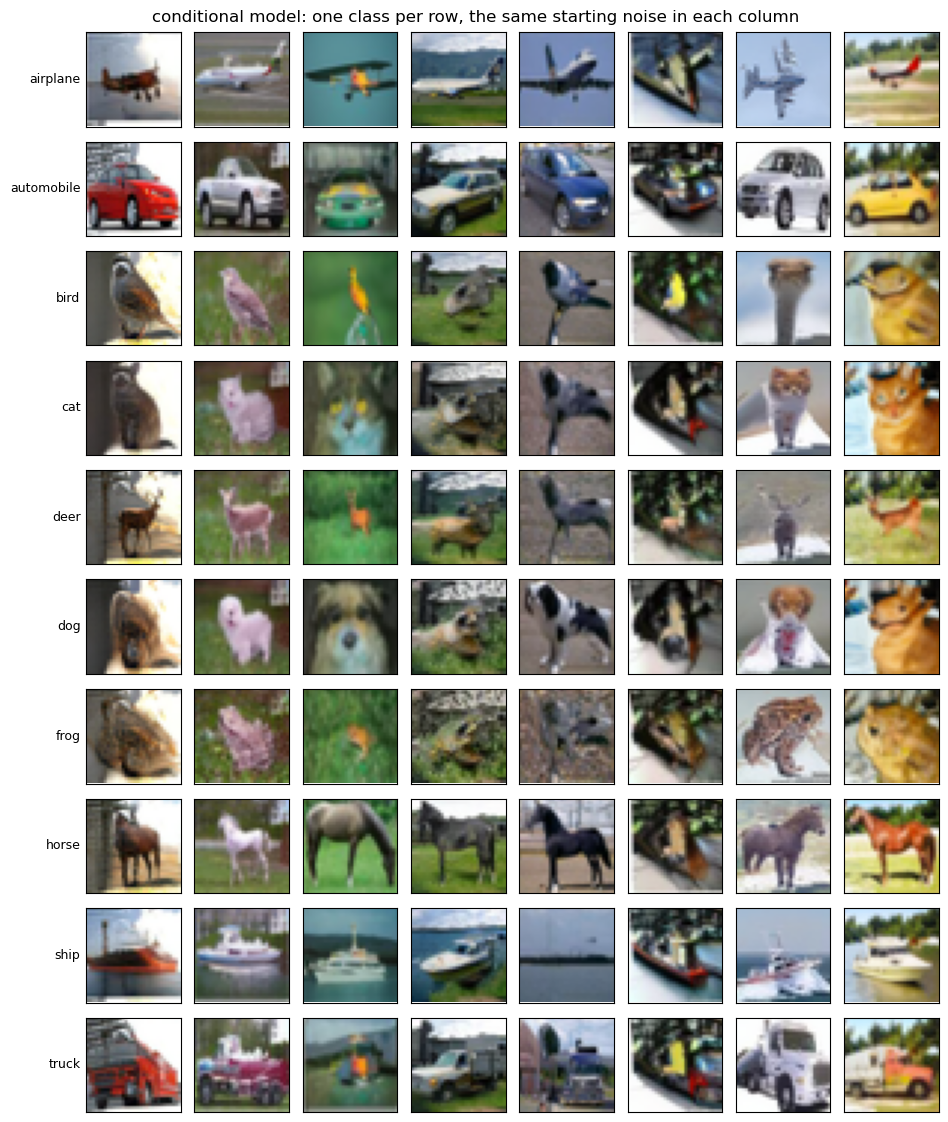
\includegraphics[width=0.6\textwidth]{figure/cond_grid_classes.png}
    \caption{Conditional samples from pretrained EDM: one class per row, the same starting noise in each column.}
    \label{fig:cond_grid}
\end{figure}

\autoref{fig:cifar_grids} compares unconditional samples (\(w = 0\)) with strongly guided samples (\(w = 4\)) from the same starting noise.
Both sets look like CIFAR-10 images, but only the guided set follows the requested classes.

\begin{figure}[H]
    \centering
    \begin{minipage}{0.48\textwidth}
        \centering
        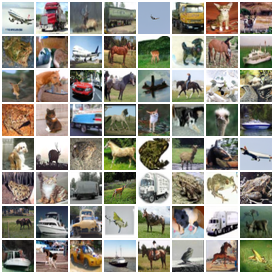
\includegraphics[width=\linewidth]{figure/cifar_grid_w0.png}
    \end{minipage}
    \hfill
    \begin{minipage}{0.48\textwidth}
        \centering
        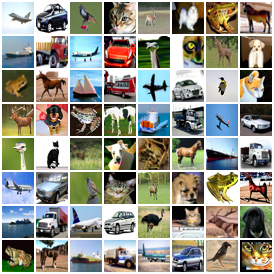
\includegraphics[width=\linewidth]{figure/cifar_grid_w4.png}
    \end{minipage}
    \caption{The first 64 of 1,000 samples at \(w = 0\) (left, unconditional, 11.5\% accuracy) and \(w = 4\) (right, 98.9\% accuracy). Image \(i\) requests class \(i \bmod 10\) in CIFAR-10 order, starting from airplane.}
    \label{fig:cifar_grids}
\end{figure}

\subsection{Inside the Sampler}

\autoref{fig:trajectories} follows three images toward the class ``cat'' from \(\sigma = 80\) down to \(\sigma = 0.002\), with the conditional model (\(w = 1\)) and with CFG at \(w = 4\), from the same seed.
The noisy image is shown as \(x / \sqrt{1 + \sigma^2}\), which keeps it in the display range.

\begin{figure}[H]
    \centering
    \begin{minipage}{0.49\textwidth}
        \centering
        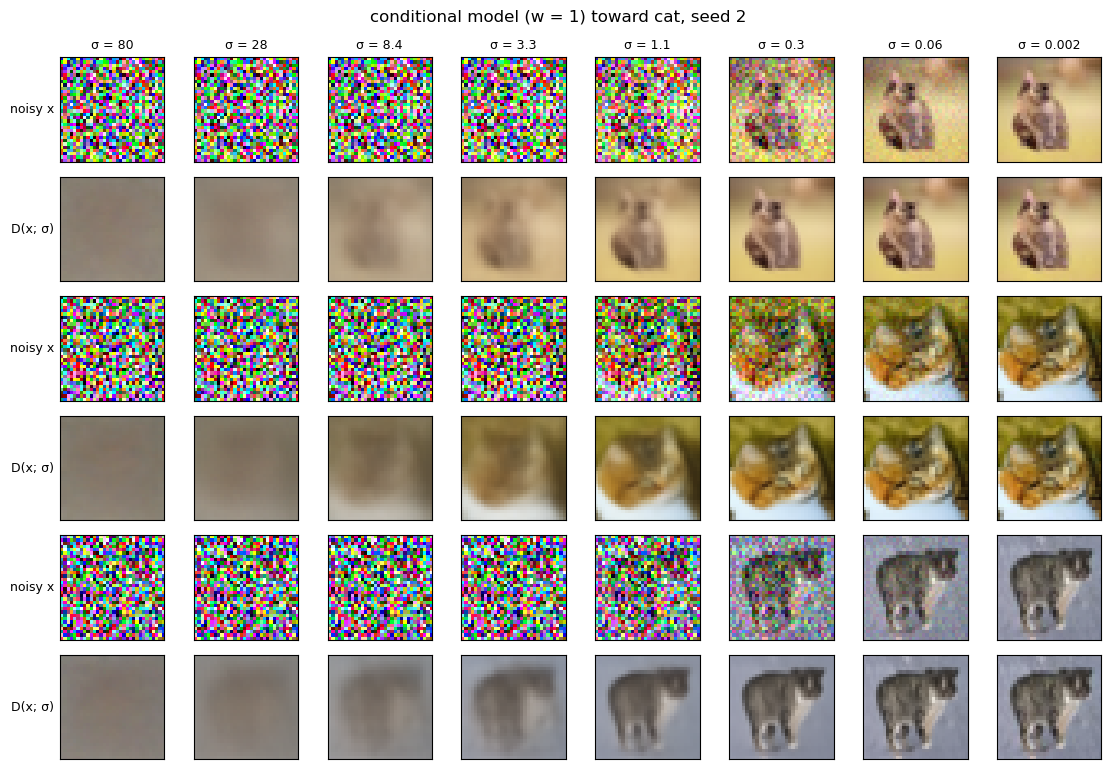
\includegraphics[width=\linewidth]{figure/trajectory_w1.png}
    \end{minipage}
    \hfill
    \begin{minipage}{0.49\textwidth}
        \centering
        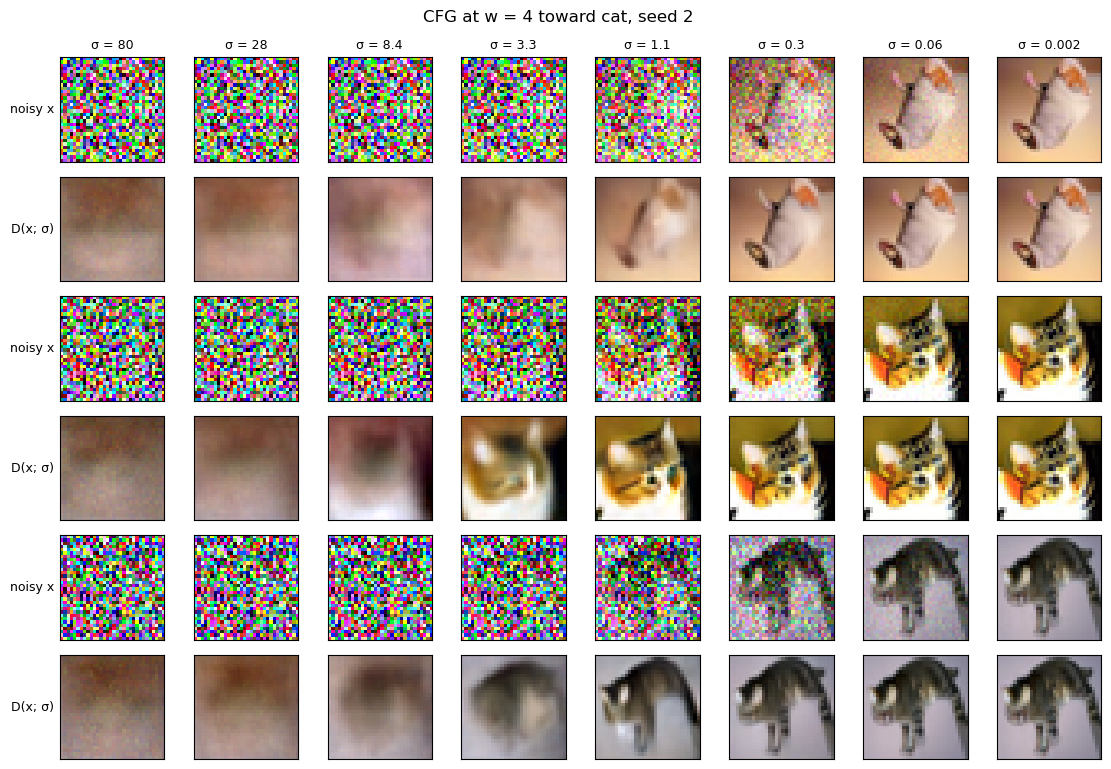
\includegraphics[width=\linewidth]{figure/trajectory_w4.png}
    \end{minipage}
    \caption{Sampling trajectories toward ``cat'' with seed 2, at \(w = 1\) (left) and \(w = 4\) (right). For each image, the upper row is the noisy image and the lower row is the denoiser's estimate \(D(x; \sigma)\), at 8 of the 18 noise levels.}
    \label{fig:trajectories}
\end{figure}

We answer the three questions of part 3 from this figure.
\begin{enumerate}
    \item \textbf{When does the class first show in \(D(x; \sigma)\)?}
    At \(\sigma = 80\) and \(28\), the estimate is a blur close to the average CIFAR-10 image.
    A rough silhouette appears around \(\sigma = 3.3\), and the cat is clearly recognizable at \(\sigma = 1.1\).
    With \(w = 4\), the estimates commit to strong colors and shapes earlier, but only one of the three images is clearly more cat-like at \(\sigma = 3.3\), so we do not see a consistent shift.
    \item \textbf{From which noise level on does the image barely change?}
    From about \(\sigma = 0.3\) on, the estimate barely changes, and at \(\sigma \le 0.06\) the noisy image and the estimate are almost identical.
    \item \textbf{How do the \(w = 4\) estimates differ at low noise?}
    They have higher contrast and saturation, with sharper but less natural features.
    The compositions also differ from the \(w = 1\) images despite the same starting noise, since the two trajectories split at high noise.
\end{enumerate}

\subsection{The CFG Sweep}

\autoref{tab:cfg_sweep} and \autoref{fig:cfg_sweep} show label accuracy, FID, and \fidclass{} against \(w\).

\begin{table}[H]
    \caption{Pretrained EDM on CIFAR-10 over the CFG sweep, with 1,000 class-balanced samples per \(w\). \fidclass{} is undefined at \(w = 0\), which ignores the requested class.}
    \label{tab:cfg_sweep}
    \centering
\begin{tabular}{cccc}
    \toprule
    \(w\) & Accuracy (\%) & FID  & \fidclass{} \\
    \midrule
    0     & 11.5          & 31.2 & N/A         \\
    1     & 95.5          & 31.3 & 112.1       \\
    1.5   & 98.7          & 31.4 & 107.6       \\
    2     & 98.8          & 33.1 & 108.9       \\
    3     & 99.5          & 36.0 & 112.4       \\
    4     & 98.9          & 39.0 & 117.5       \\
    \bottomrule
\end{tabular}

\end{table}

\begin{figure}[H]
    \centering
    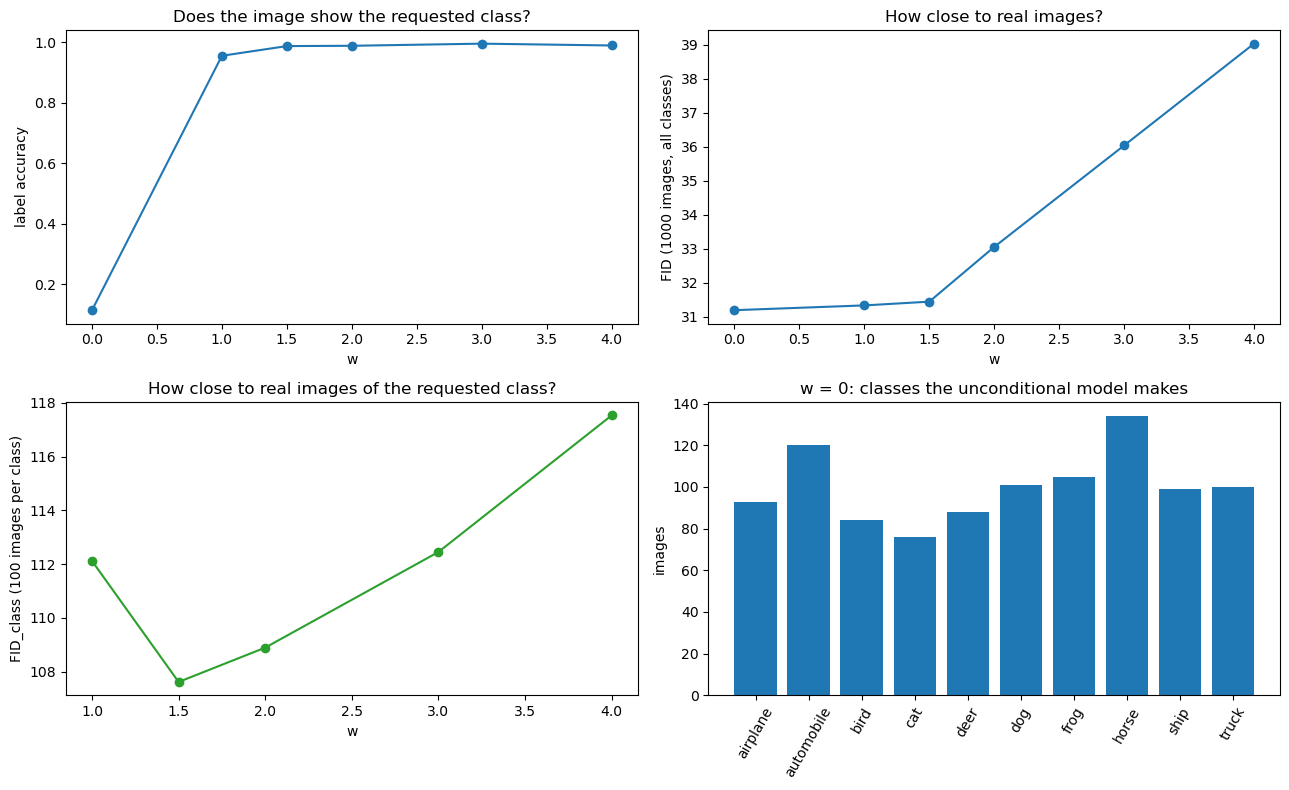
\includegraphics[width=0.75\textwidth]{figure/cfg_sweep_plots.png}
    \caption{Label accuracy (top left), FID (top right), and \fidclass{} (bottom left) against \(w\), and the classes the unconditional model makes at \(w = 0\) according to the classifier (bottom right).}
    \label{fig:cfg_sweep}
\end{figure}

Accuracy rises from near chance (11.5\%) to 95.5\% at \(w = 1\) and saturates near 99\% from \(w = 1.5\) on.
FID stays relatively flat up to \(w = 1.5\) and then grows to 39.0 at \(w = 4\), because guidance makes the images of each class more alike, so the whole set has less variety than the training images.
\fidclass{} is lowest at \(w = 1.5\) (107.6) and grows after that, so beyond \(w = 1.5\) the images get no more recognizable but drift further from real images of their class.
\fidclass{} uses only 100 images per class, so it is much higher than the all-class FID and should only be compared across \(w\).
At \(w = 0\), the unconditional model covers all ten classes, but not uniformly.
Horses and automobiles are over-represented, and cats and birds are under-represented.

\subsection{Small CFG Networks on CIFAR-10 Subsets}

\autoref{tab:subset_fid} and \autoref{fig:subset_loss_fid} show that the training loss falls steadily for both subset sizes, while FID rises after the first snapshot.

\begin{table}[H]
    \caption{FID across snapshots for the subset networks, each from 1,000 unconditional samples.}
    \label{tab:subset_fid}
    \centering
\begin{tabular}{lccccc}
    \toprule
                    & \multicolumn{5}{c}{Update}                   \\
    \cmidrule(lr){2-6}
    Training images & 4,000 & 8,000 & 12,000 & 16,000 & 20,000     \\
    \midrule
    100             & 75.3  & 92.4  & 106.1  & 106.6  & 110.5      \\
    1,000           & 93.9  & 110.4 & 124.9  & 125.8  & 132.8      \\
    \bottomrule
\end{tabular}

\end{table}

\begin{figure}[H]
    \centering
    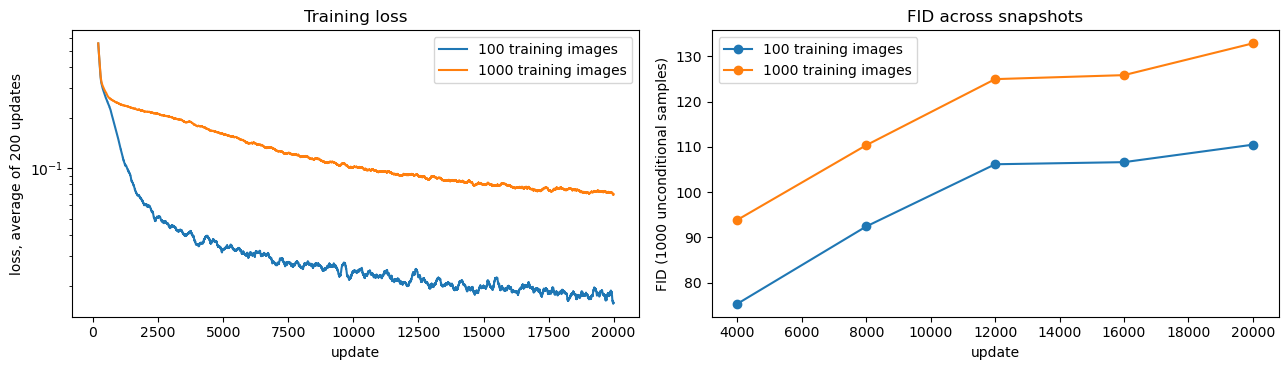
\includegraphics[width=\textwidth]{figure/subset_loss_fid.png}
    \caption{Training on 100 and 1,000 CIFAR-10 images: training loss averaged over 200 updates (left) and FID across snapshots (right).}
    \label{fig:subset_loss_fid}
\end{figure}

\autoref{fig:nearest} explains the rising FID.
In the 100-image network, the median distance from its samples to the nearest training image is 1.2, compared with 23.7 for real test images, and nearly every sample is a copy of a training image.
The 1,000-image network memorizes much less (14.5 for samples against 21.3 for test images).
As training continues, both networks reproduce their small training sets more closely, so their samples move away from the full CIFAR-10 distribution that FID compares them with.

\begin{figure}[H]
    \centering
    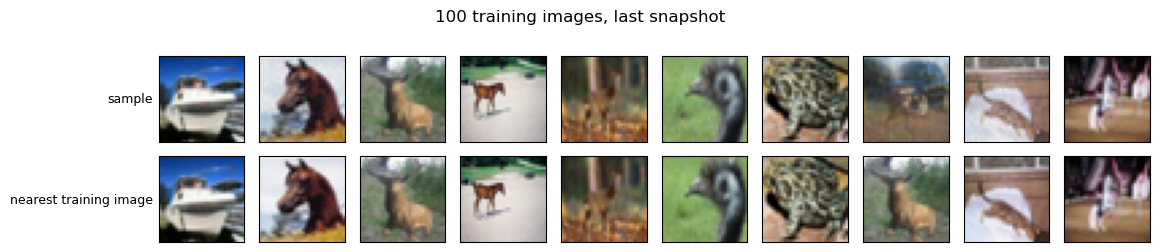
\includegraphics[width=0.9\textwidth]{figure/nearest_subset100.png}
    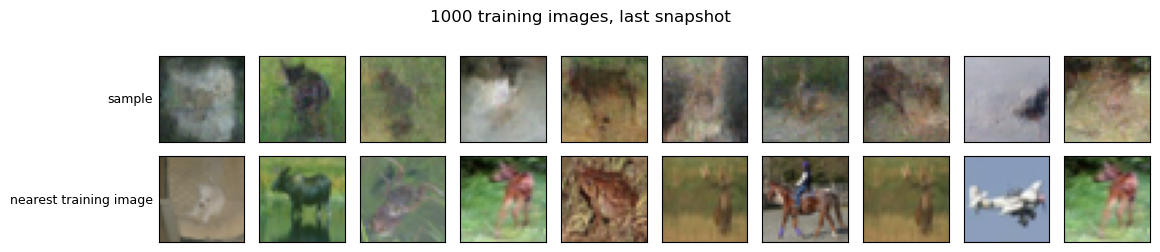
\includegraphics[width=0.9\textwidth]{figure/nearest_subset1000.png}
    \caption{Samples from the last snapshot (upper rows) next to their nearest training images (lower rows), for the 100-image network (top) and the 1,000-image network (bottom).}
    \label{fig:nearest}
\end{figure}

\autoref{fig:subset_cfg} shows CFG with one network, from the same starting noise in each column.
For the 100-image network, accuracy rises from 7\% at \(w = 0\) to 93\% at \(w = 1\) and 100\% at \(w \ge 2\).
These high accuracies come from memorization: the samples are copies of correctly labeled training images.
For the 1,000-image network, accuracy rises more slowly, from 15\% to 38\%, 69\%, and 83\% at \(w = 1, 2, 4\), so guidance does more of the work.
Each accuracy comes from only 100 samples.

\begin{figure}[H]
    \centering
    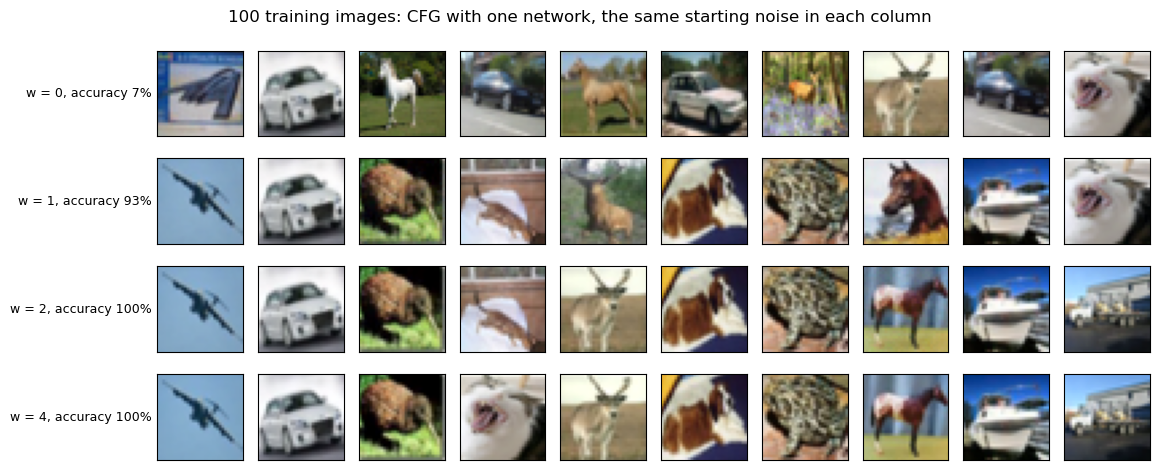
\includegraphics[width=0.8\textwidth]{figure/subset100_cfg.png}
    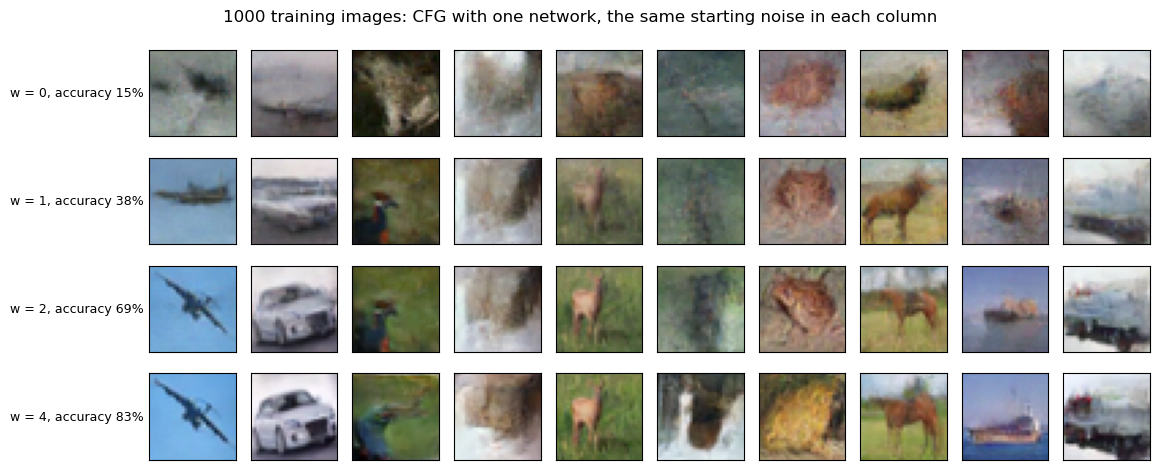
\includegraphics[width=0.8\textwidth]{figure/subset1000_cfg.png}
    \caption{CFG with the 100-image network (top) and the 1,000-image network (bottom), at \(w = 0, 1, 2, 4\), with the same starting noise in each column.}
    \label{fig:subset_cfg}
\end{figure}

\subsection{From-Scratch CFG on MNIST}

\autoref{tab:mnist} and \autoref{fig:mnist} show that the CFG pattern carries over to a network we trained from scratch on a different dataset.

\begin{table}[H]
    \caption{One-network CFG on MNIST, with 1,000 samples per \(w\). FID uses the frozen digit classifier's features (\autoref{sec:data}). NFE (network evaluations per image) doubles for \(w \notin \{0, 1\}\), where each step needs both the conditional and the unconditional estimate.}
    \label{tab:mnist}
    \centering
\begin{tabular}{cccc}
    \toprule
    \(w\) & Accuracy (\%) & FID   & NFE \\
    \midrule
    0     & 9.8           & 164.9 & 16  \\
    1     & 98.3          & 39.4  & 16  \\
    2     & 100.0         & 67.2  & 32  \\
    4     & 100.0         & 122.1 & 32  \\
    \bottomrule
\end{tabular}

\end{table}

\begin{figure}[H]
    \centering
    \begin{minipage}{0.4\textwidth}
        \centering
        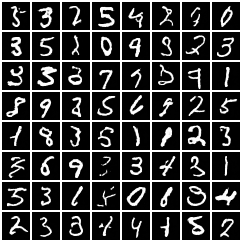
\includegraphics[width=\linewidth]{figure/mnist_grid_w0.png}
    \end{minipage}
    \hspace{0.05\textwidth}
    \begin{minipage}{0.4\textwidth}
        \centering
        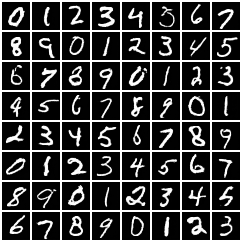
\includegraphics[width=\linewidth]{figure/mnist_grid_w1.png}
    \end{minipage}
    \caption{The first 64 MNIST samples at \(w = 0\) (left) and \(w = 1\) (right).}
    \label{fig:mnist}
\end{figure}

At \(w = 0\), the network draws clean digits, but they ignore the requested label (9.8\% accuracy).
At \(w = 1\), accuracy reaches 98.3\% and FID is lowest (39.4).
Guidance beyond \(w = 1\) adds the last 1.7 points of accuracy but nearly doubles FID by \(w = 2\) and triples it by \(w = 4\).
The FID of 164.9 at \(w = 0\) is unexpectedly high for samples that look like clean digits, and we will investigate it next.

\subsection{A Short Run of Full EDM Training}

\autoref{fig:full_run} shows EDM's \texttt{train.py} on all 50,000 CIFAR-10 images.
We stopped the run after 2.9 hours, once it had written three snapshots (0, 502, and 1,004 kimg).

\begin{figure}[H]
    \centering
    \begin{minipage}{0.48\textwidth}
        \centering
        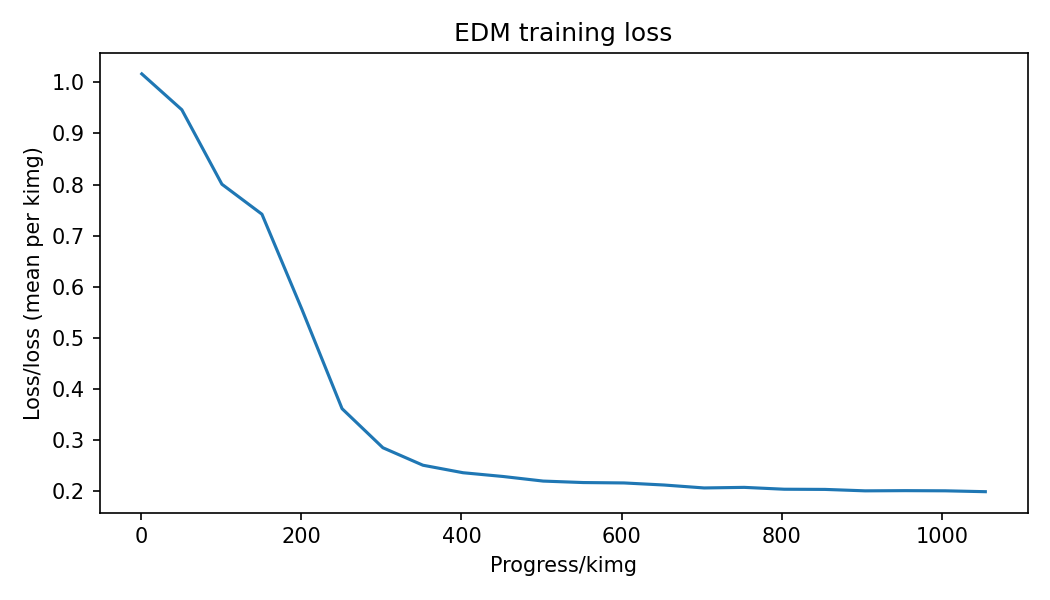
\includegraphics[width=\linewidth]{figure/loss_curve.png}
    \end{minipage}
    \hfill
    \begin{minipage}{0.48\textwidth}
        \centering
        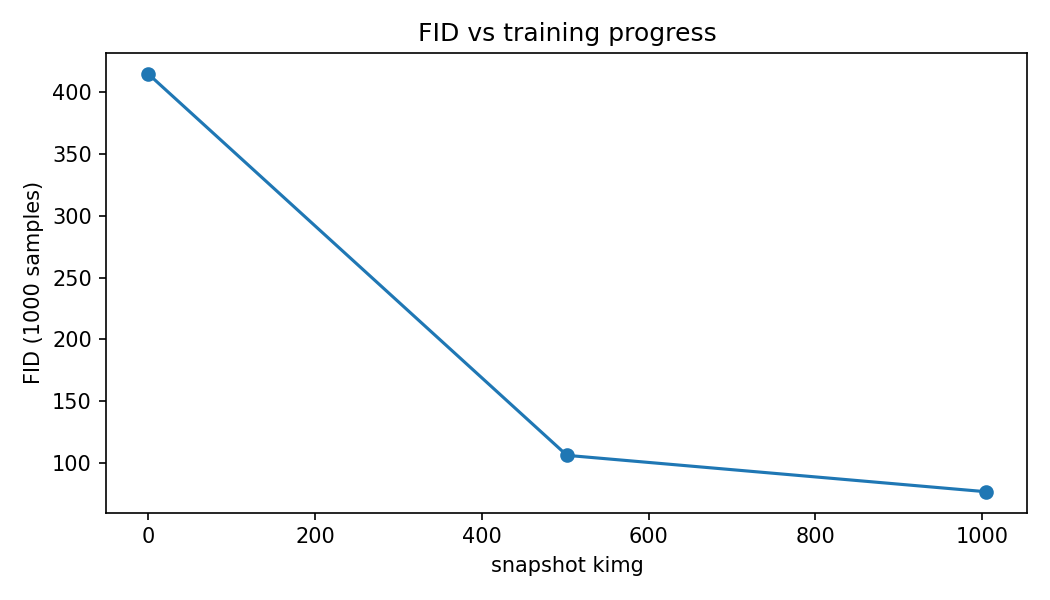
\includegraphics[width=\linewidth]{figure/fid_vs_kimg.png}
    \end{minipage}
    \caption{Full EDM training on one GTX 1080 Ti: training loss (left) and FID across snapshots from 1,000 unconditional samples each (right).}
    \label{fig:full_run}
\end{figure}

The loss falls from 1.02 to about 0.20, with most of the drop before 300 kimg.
FID falls from 414.7 (untrained) to 106.2 at 502 kimg and 76.9 at 1,004 kimg.
For comparison, the pretrained unconditional network scores 31.2 under the same protocol (\(w = 0\) in \autoref{tab:cfg_sweep}).
Our run covers about 0.5\% of EDM's 200-million-image schedule, and FID is still falling.

\section{Discussion}

\paragraph{Guidance costs more per class than overall}
On the pretrained model, raising accuracy from 11.5\% to 99.5\% costs only 4.8 FID points (31.2 to 36.0 at \(w = 3\)).
However, looking at the per-class breakdown, we see that \fidclass{} is lowest at \(w = 1.5\) and grows steadily after, so the all-class FID understates how much variety guidance removes within each class.
Based on both measures, we would choose \(w = 1.5\) for this model.

\paragraph{On small data, more training means more memorization}
Both subset networks get worse in FID while their loss improves.
This is due to memorization: the 100-image network's samples are near-copies of its training images, so longer training only reproduces them more closely.
The same copies also make its CFG accuracies look excellent, so label accuracy alone cannot tell control from memorization.

\paragraph{The pretrained FID is a matter of compute}
Our short full training run uses the same network and recipe as the pretrained model, and its FID is still falling at 76.9.
The gap to the pretrained 31.2 comes from the remaining 99.5\% of the training schedule, not from a different recipe.

\paragraph{Limitations}
\begin{itemize}
    \item All FIDs use 1,000 samples instead of the published 50,000, so absolute values are inflated and only comparisons within a table are meaningful.
    \item The MNIST FID uses classifier features instead of Inception features, so it cannot be compared with the CIFAR-10 numbers.
    \item The subset CFG accuracies come from 100 samples each, so they carry several points of sampling noise.
    \item Our observations on the trajectories come from three images and one seed.
\end{itemize}

\section{Conclusion}

We reproduced sampling with EDM's pretrained CIFAR-10 networks, looked inside its Heun sampler through trajectories, and measured a CFG sweep with label accuracy, FID, and per-class FID.
We also trained CFG networks on small CIFAR-10 subsets and from scratch on MNIST, and ran the start of EDM's full training.
The results agree with the claims of the EDM and CFG papers: guidance buys adherence to the class at a mild cost in FID, and that cost is concentrated within each class.
This also warns us for the capstone that on small training sets, guidance mostly selects memorized images rather than providing real control.
Next, we plan to carry these tools to continuous diffusion models for text, where CFG will again serve as the baseline for controlling what the model generates.

%%%%%%%%%%%%%%%%%%%%%%%%%%%%%%%%%%%%%%%%%%%%%%%%%%%%%%%%
%%%% Reference / Bibliography
%%%%%%%%%%%%%%%%%%%%%%%%%%%%%%%%%%%%%%%%%%%%%%%%%%%%%%%%

\makereference

\bibliography{reference}
\bibliographystyle{style/dsc180bibstyle}

%%%%%%%%%%%%%%%%%%%%%%%%%%%%%%%%%%%%%%%%%%%%%%%%%%%%%%%%
%%%% Appendix
%%%%%%%%%%%%%%%%%%%%%%%%%%%%%%%%%%%%%%%%%%%%%%%%%%%%%%%%

\clearpage
\makeappendix

\subsection{AI Use}

AI (Hermes Agent with models GLM 5.3 Flash and Claude Opus 5.5) was used to help understand the EDM paper and codebase, adapt and debug the code, monitor and launch GPU jobs on DSMLP, refine the language of our own drafts, keep the README current, and cross-check our interpretations of results.
The experimental design, first drafts, result interpretations, most of the \LaTeX{} and all final decisions are our own, and every reported number was checked against the saved outputs.
The full summary, representative prompts and validation steps are in \href{https://github.com/vishudhshah/edm/blob/main/AI_USE.md}{\texttt{AI\_USE.md}} in the repository.

\end{document}
